\begin{figure*}
  \begin{minipage}{.5\textwidth}
    \centering
    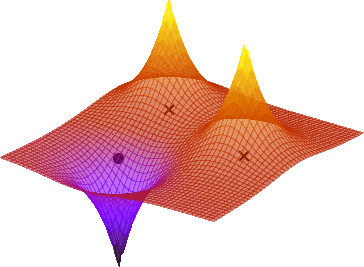
\includegraphics[width=\linewidth]{influence_map.png}
  \end{minipage}%
  \begin{minipage}{.5\textwidth}
    \centering
    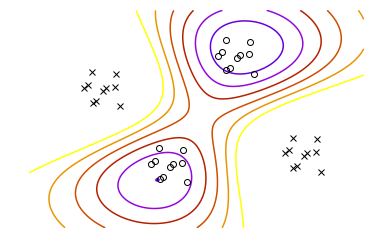
\includegraphics[width=\linewidth]{decision_boundary.png}
  \end{minipage}
  \caption{
    Left side shows on the vertical axis the influence level of the point on the 2d plane from two positive points drawn  with \textbf{x} markers and of one negative points marked with \textbf{o}. On the right pane, the solid line reprensents the decision boundary and the dashed lines represents the contour levels of the decision function with learned using an RBF kernel.
  }
\end{figure*}

\section{Kernel methods}

The previous section introduced the linear SVM classifier. The linear SVM, as we saw, allows us the find the best seperating hyperplane between two linearly seperable classes of a dataset. In this section we introduce the concept of kernels, allowing us to learn non linear decision boudaries, continuing with the Mercer theorem and kernel trick, results from functional analysis allowing us to use the newly introducd ideas of kernels with the previously introduces agorithm, with only light modifications.

\subsection{Non linearly separable data}

Very often, the decision boundary one is trying to learn is in it's nature non-linear. One trick that is often used in order to use linear learning algorithms is to add one or several dimensions to the data points by applying a non linear function of the coordinates of the point, to then learn the separating hyperplane in the projhected space. This method is known as features engineering, because we add engineered features to our data points.


This approach would be very simple to implement in our current algorithm. Let $\phi : \mathcal{X} \rightarrow \mathcal{V}$ be a non linear transformation from our original space $\mathcal{X}$ to some higer dimensional pre Hilbert space $\mathcal{V}$. A pre Hilbert space is a generalization of a Euclidean space, the geometrical space we are used to. Saying that the image of the projection should be a pre Hilbert space simply means that the image set is equiped with a scalar product, needed for our training algorithm. We can now modify the previously introduced algorithm by replacing simply every dot product by the scalar product on the projected points in the $\mathcal{V}$ space, namely $\langle \phi(\cdot), \phi(\cdot)\rangle _{\mathcal{V}}$.


In order to better understand kernels and the kernel trick, let's follow the example of polynomial projection of degree $d$, in which every point is projected to a vector containing every monomial of degree $d$. For instance, choosing $d = 2$ together with a $2$ dimensional input space leads to the projection $\phi : \mathbb{R}^2 \rightarrow \mathbb{R}^4$ defined as

\begin{equation*}
    \phi(x_1, x_2) \mapsto (x_1^2, x_2^2, x_1x_2, x_2x_1)
\end{equation*}

This representation, while adding more separation capabilities has the problem that the image feature space grows at an exponential rate together with $d$, making the choice of a larger $d$ prohibitivly expensive in terms of space usage. Though, the margin maximization algorithm only uses the scalar product of the observations in the feature space, which is simply the dot product of the mapped vectors. The following equations show that the projection in the high dimensional space is not required to the computation of the scalar product

\begin{equation*}
  \begin{aligned}
    \phi(x) \cdot \phi(\tilde{x})
    &= x_1^2\tilde{x}_1^2 + x_2^2\tilde{x}_2^2 + 2x_1x_2\tilde{x}_1\tilde{x}_2\\
    &= \left(x \cdot \tilde{x}\right)^2 \\
    &=: k(x, \tilde{x})
  \end{aligned}
\end{equation*}

We call $k(\cdot, \cdot) : \mathbb{R}^2 \times \mathbb{R}^2 \rightarrow \mathbb{R}$ the kernel representation of the scalar product in the space $\phi(\mathbb{R}^2)$. One can generalize this idea to any polynomial degree $d$ as shown in \textcolor[rgb]{1,0,0}{ref?}, making the computation of the scalar product in the $d$-th monomial space as trivial as computing the scalar product in the original space.

\subsection{Kernel trick}

We have seen in the previous example, that it is sometimes possible to find a function $k :\mathcal{X} \times \mathcal{X} \rightarrow \mathbb{R}$ with $k(x, x') = \langle \phi(x), \phi(x')\rangle _{\mathcal{V}}$ for some projection $\phi : \mathcal{X} \rightarrow \mathcal{V}$. With these special functions, it is possible by only lightly modifying our original algorithm to run the learning algorithm in another pre Hilbert space without the computational cost of projecting our data in this other space. This is called the kernel trick.

We will now change our point of view, and try to define the properties defining the class of functions being the representation of a scalar product of the projection of its inputs in another vector space. This means, which properties must hold for $k$ in order for a $\phi$ to exist with the correspondance property.

Let $k :\mathcal{X} \times \mathcal{X} \rightarrow \mathbb{R}$ with $k(x, x') = \langle \phi(x), \phi(x')\rangle _{\mathcal{V}}$ for some projection $\mathcal{X} \rightarrow \mathcal{V}$, because $\langle \cdot, \cdot\rangle _{\mathcal{V}}$ is a scalar product, the following properties must hold

\begin{itemize}
\item \textit{Symmetry}
  \begin{equation*}
    \begin{aligned}
      & \forall y_1, y_2 \in \mathcal{V}.\ 
      \langle y_1, y_2\rangle _{\mathcal{V}} = \overline{\langle y_2, y_1\rangle _{\mathcal{V}}} & \Rightarrow\\
      & \forall y_1, y_2 \in \phi(\mathcal{X}).\ 
      \langle y_1, y_2\rangle _{\mathcal{V}} = \overline{\langle y_2, y_1\rangle _{\mathcal{V}}} & \Rightarrow\\
      &\forall x_1, x_2 \in \mathcal{X}.\ 
      \langle \phi(x_1), \phi(x_2)\rangle _{\mathcal{V}} = \overline{\langle \phi(x_2), \phi(x_1)\rangle _{\mathcal{V}}} &\Rightarrow\\
      &\forall x_1, x_2 \in \mathcal{X}.\ 
         k\left(x_1, x_2\right) = \overline{k\left(x_2, x_1\right)}
    \end{aligned}
  \end{equation*}

\item \textit{Positive definitness} Positive definitness of a kernel is a stronger property than the one required for the positive definiteness in the features space. A kernel is said to be positive definite if for every $\alpha_1, ..., \alpha_n \in \mathbb{R}$ following inequality holds
  \begin{equation*}
    \sum_{i,j=1}^n\alpha_i\alpha_jk\left(x_i, x_j\right) \geq 0
  \end{equation*}
\end{itemize}

We will show by construction, that these properties are sufficient to the proof of the existence of the desired space. The literature contains several examples of vector spaces and projections with the desired property. We will here proove the existence of such a space by construction.

Let $k : \mathcal{X} \times \mathcal{X} \rightarrow \mathbb{R}$ be symmetrical and positive definite, and $\mathbb{R}^{\mathcal{X}}$ be the set of functions from a non empty set $\mathcal{X}$ to $\mathbb{R}$. We define the reproducing kernel map as follow

\begin{equation}
  \begin{aligned}
    \phi : \mathcal{X} \rightarrow \mathcal{H}\\
    \mathbf{x} \mapsto k(\cdot, \mathbf{x})
  \end{aligned}
\end{equation}

We now show how the mapped observations of the training set $\left\{k\left(\cdot, \mathbf{x}_1\right), ..., k\left(\cdot, \mathbf{x}_n\right)\right\}$ spans a Hilbert space in which the reproducing property hold with the scalar defined on the span set $\langle k\left(\cdot, \mathbf{x}_i\right), k\left(\cdot, \mathbf{x}_j\right)\rangle = k\left(\mathbf{x}_i, \mathbf{x}_j\right)$ and its canonical derivation for the spanned space

\begin{equation*}
  \begin{aligned}
    \langle f, g\rangle 
    &= \langle \sum_{i=1}^n\alpha_ik(\cdot, \mathbf{x}_i), \sum_{j=1}^n\beta_jk(\cdot, \mathbf{x}_j)\rangle \\
    &= \sum_{i,j=1}^n\alpha_i\beta_j \langle k\left(\cdot, \mathbf{x}_i\right), k\left(\cdot, \mathbf{x}_j\right)\rangle \\
    &= \sum_{i,j=1}^n\alpha_i\beta_j k\left(\mathbf{x}_i, \mathbf{x}_j\right)
  \end{aligned}
\end{equation*}

Positive definitness, bilinearity and symmetry can all be trivially derived from the definition of this scalar product together with the symmetry and positive definitness of the kernel function. Then attentive reader will notive that the functions $\left\{k\left(\cdot, x_1\right), ..., k\left(\cdot, x_n\right)\right\}$ must nost necessarily be linearly independant, leading to a non unqiue mapping from $f$ to the coefficients $\alpha_1, ..., \alpha_n$. To see that this doesn't imply the ill definitness of the defined scalar product, we note that

\begin{equation*}
  \langle f, g\rangle = \sum_{j=1}^n\beta_j f\left(\mathbf{x}_j\right)
\end{equation*}

and by symmetry

\begin{equation*}
  \langle f, g\rangle = \langle g, f\rangle = \sum_{i=1}^n\alpha_i g\left(\mathbf{x}_i\right)
\end{equation*}

Which shows that the scalar product does not depend on the choice of coefficients for the functions $f$ and $g$ confirming the scalar product is well defined. Thus, the previously defined scalar product, together with the norm $|f| = \sqrt{\langle f, f\rangle }$ define a valid Hilbert space and the correspondance property holds

\begin{equation*}
  \begin{aligned}
    \langle \phi(\mathbf{x}_i), \phi(\mathbf{x}_j)\rangle =\ &\langle k\left(\cdot, \mathbf{x}_i\right), k\left(\cdot, \mathbf{x}_j\right)\rangle \\
    =\ &k(\mathbf{x}_i, \mathbf{x}_j)
  \end{aligned}
\end{equation*}

Now that we have presented the kernel trick as well as the existence of a corresponding Hilbert space, the next section will focus on finding and creating useful kernels, as well as presenting some classical kernels.

\subsection {Some useful kernels}

We have defined in the last section what kernels are and how we can modify our algorithm to learn non-linear boundaries in our data. What we have omited so far is how is one supposed to choose develop or choose a kernel when facing a practical problem.

One first way to choose a kernel is by using existing knowledge about the shape the decision boundary should have. Let's recall the equation of the decision boundary defined by the learned parameters using the kernel $k$

\begin{equation*}
  \mathscr{H} = \left\{\mathbf{x} \in \mathbb{R}^n\ |\ \sum_{\mathbf{x}_i \text{ is SV}}\alpha_iy_ik\left(\mathbf{x}, \mathbf{x}_i\right) + b = 0\right\}
\end{equation*}

For illustration, if we choose the kernel to be a polynomial kernel of degree $2$, meaning $k\left(\mathbf{x}, \mathbf{\tilde{x}}\right) = \left(\mathbf{x} \cdot \mathbf{\tilde{x}} + 1\right)^2$, we can refine the definition of the decision boundary as the set of every $\mathbf{x} \in \mathbb{R}^2$ for which following holds

\begin{equation*}
  \begin{aligned}
    0 &=\ \left(w \cdot \mathbf{x} + 1\right)^2 + b\\
      &=\ \left(w_1x_1 + w_2x_2 + 1\right)^2 + b\\
      &=\ (w_1x_1)^2 + (w_2x_2)^2 + 2w_1x_1w_2x_2 + w_1x_1 + w_2x_2 + 1 + b\\
      &=\ \mathbf{x}^T\begin{bmatrix}w_1^2 & w_1w_2\\ w_1w_2 & w_2^2\end{bmatrix}\mathbf{x} + w \cdot \mathbf{x} + 1 
  \end{aligned}
\end{equation*}

The decision boundary formed by this equation is called a quadric, the generalization of a conic section, which takes a shape from a known set of different kind of solutions. Thus, if one knows a quadric decision boundary is needed, then using a polynomial kernel of degree $2$ will learn the proper parameters of the quadric.

We have seen how previous knowledge on the shape of the decision boundary can lead to the choice of a particular kernel. Unfortunately, it is often the case that the best kind of decision boundary can't be determined. Thankfully, there is still a way to use domain knowledge about the problem to choose a kernel that will best help training a performant classifier.


In order to incorporate this other kind of domain knowledge, we have to look at kernels, not as the computations of a scalar product in some feature space, but as a similarity measurement. Taking this point of view, the kernel trick becomes a way to find the proper Hilbert space in which one's definition of similarity defines a scalar proper product, letting us use the Support Vector Machine machinery as a way to train a classifier based on our definition of similarity.

What do we mean by similarity? Let's first write down a more geometrical  definition of the euclidean scalar product in $\mathbb{R}^n$, the inner product 

\begin{equation*}
  \mathbf{x} \cdot \mathbf{\tilde{x}} = \|\mathbf{x}\|\|\mathbf{\tilde{x}}\|\text{cos}\left(angle\left(\mathbf{x}, \mathbf{\tilde{x}}\right)
  \right)
\end{equation*}

This equivalent definition of the euclidean scalar product makes it more visible what the underlying notion of similarity of the euclidean scalar product is measured by the angle between the two vectors, scaled by their length. A similar kernel often used is the cosine similarity kernel, defined as

\begin{equation*}
  k(\mathbf{x}, \mathbf{\tilde{x}}) = \frac{\mathbf{x} \cdot \mathbf{\tilde{x}}}{\|\mathbf{x}\|\|\mathbf{\tilde{x}}\|} = \text{cos}\left(angle\left(\mathbf{x}, \mathbf{\tilde{x}}\right)\right)
\end{equation*}

This notion of similarity will thus compare observations by first normalizing them to then compare the directions of the vectors. This similarity measure is often used in the context of text classification, where each entry of the vector corresponds to the number of occurences of a word in a text. The normalization will transform count of occurences in frequencies, thus having a similarity based on the relative importance of each word, independantly of the length of the text.

Cosine similarity is an interesting similarity, but one natural way to reason about similarity of points is their distance from one another. The next kernel we introduce incorporates the notions of distance as a similarity measurement, is called the Radial Basis Function kernel and is defined as followed for some hyperparameter $\sigma \in \mathbb{R}$

\begin{equation*}
  k(\mathbf{x}, \mathbf{\tilde{x}}) = \text{exp}\left(-\frac{\|\mathbf{x} - \mathbf{\tilde{x}}\|^2}{\sigma^2}\right)
\end{equation*}

This kernel contains the idea that similarity between two observations should decay exponentially with the distance between the two vectors. This kernel isn't only a good model of our notion of similarity, but it also has interesting properties when used with the Support Vector Machines training algorithm.

Let's first recall what was the decision function that was learned by the algorithm

\begin{equation*}
  f\left(x\right) = sgn\left(\sum_{\mathbf{x}_i \text{ is SV}}\alpha_iy_ik\left(\mathbf{x}, \mathbf{x}_i\right) + b\right)
\end{equation*}

We evaluate the sign of a linear combination of the similarity of the current observation to the support vectors. One can see understand each support vector as a point of influence in the direction of the class it belongs to, with it's influence intensity exponentially decaying with the distance. The observation will then be classified by taking a weighted sum of the influence of each support vector and verifying if it is over or under some threshold $b$. This intuition can be visualised in figure 2 where we show the influence map built by two points on in a one dimensional space as well as a decision boundary learned using a radial basis function kernel.

We have shown with three examples how previous knowledge can help train high quality classifiers. Because we had to omit many interesting concepts of choice of kernel, the reader is invited to consult further resources to learn about more mechanical ways to construct kernels \textcolor[rgb]{1,0,0}{ref linear combination, partial kernels...} but also about invariance incorporation \textcolor[rgb]{1,0,0}{ref} or advanced approach in kernel design for solving modern complex problems \textcolor[rgb]{1,0,0}{ref}.

%%% Local Variables:
%%% mode: latex
%%% TeX-master: "learning_with_kernels"
%%% End:
